\documentclass[a4paper, 12pt]{report}
\renewcommand{\baselinestretch}{1.5}
\usepackage[utf8]{inputenc} % Change according your file encoding
\usepackage{graphicx}
\usepackage{url}
\usepackage{geometry}
\usepackage{titlesec}
\usepackage{listings}

\usepackage{tabularx}

\geometry{
 left=2.4cm,
 top=2.5cm,
 bottom=2.5cm,
 right=1.4cm
 }
 
\usepackage{fancyhdr}
\pagestyle{fancy}
\fancypagestyle{IHA-fancy-style}%
\fancyhf{}%

\lhead{}
\rhead{\fontsize{10pt}{10pt}\selectfont AUTOMATIC ATTENDANCE SYSTEM USING FACE RECOGNITION }
\rfoot{\fontsize{10pt}{10pt}\selectfont Sree Narayana Gurukulam College of Engineering}
\cfoot{\thepage}
\lfoot{\fontsize{10pt}{10pt}\selectfont Department of Computer Applications}
\renewcommand{\headrulewidth}{0.4pt}
\renewcommand{\footrulewidth}{0.4pt}

\pagestyle{fancy}
\lhead{}
\rhead{\fontsize{10pt}{10pt}\selectfont AUTOMATIC ATTENDANCE SYSTEM USING FACE RECOGNITION}
\rfoot{\fontsize{10pt}{10pt}\selectfont Sree Narayana Gurukulam College of Engineering}
\cfoot{\thepage}
\lfoot{\fontsize{10pt}{10pt}\selectfont Department of Computer Applications}
\renewcommand{\headrulewidth}{0.4pt}
\renewcommand{\footrulewidth}{0.4pt}
\fancypagestyle{IHA-fancy-style}{%
\fancyhf{}%
\lhead{}
\rhead{\fontsize{10pt}{10pt}\selectfont AUTOMATIC ATTENDANCE SYSTEM USING FACE RECOGNITION }
\rfoot{\fontsize{10pt}{10pt}\selectfont Sree Narayana Gurukulam College of Engineering}
\cfoot{\thepage}
\lfoot{\fontsize{10pt}{10pt}\selectfont Department of Computer Applications}
%\fancyhead[LE,RO]{\slshape \rightmark}
%\fancyhead[LO,RE]{\slshape \leftmark}
%\fancyfoot[C]{\thepage of \pageref{LastPage}}%
\renewcommand{\headrulewidth}{0.4pt}
\renewcommand{\footrulewidth}{0.4pt}
}


\fancypagestyle{plain}{
\fancyhf{}%
\lhead{}
\rhead{\fontsize{10pt}{10pt}\selectfont AUTOMATIC ATTENDANCE SYSTEM USING FACE RECOGNITION }
\rfoot{\fontsize{10pt}{10pt}\selectfont Sree Narayana Gurukulam College of Engineering}
\cfoot{\thepage}
\lfoot{\fontsize{10pt}{10pt}\selectfont Department of Computer Applications}
%\fancyfoot[C]{\thepage of \pageref{LastPage}}%
\renewcommand{\headrulewidth}{0.4pt}%
\renewcommand{\footrulewidth}{0.4pt}%
}
\usepackage{enumitem}
\begin{document}

\begin{titlepage}
	\centering
	\vspace{0.4cm}
	{\bfseries\fontsize{16pt}{16pt}\selectfont AUTOMATIC ATTENDANCE SYSTEM USING FACE RECOGNITION \par}
	\vspace{.6cm}
	{\bfseries\fontsize{12pt}{12pt}\selectfont PROJECT REPORT \par}
	\vspace{.6cm}
		{\fontsize{12pt}{12pt}\selectfont\bfseries Submitted by \par}
		
	\vspace{.6cm}
	{\fontsize{14pt}{14pt}\selectfont\bfseries ABIN C JOSE}
		{\fontsize{12pt}{12pt}\selectfont\bfseries (Reg.No: LSNG17MCA007)\par}
	\vspace{.6cm}
	{\fontsize{14pt}{14pt}\selectfont\bfseries\hspace{3cm} AMRUTHA SURENDRAN}
		{\fontsize{12pt}{12pt}\selectfont\bfseries (Reg.No: KVE17MCA004)\par}
	\vspace{.6cm}
	{\fontsize{14pt}{14pt}\selectfont\bfseries VARNA B LAL}
		{\fontsize{12pt}{12pt}\selectfont\bfseries (Reg.No: KVE17MCA023)\par}
	\vspace{.6cm}
	
	
	{\fontsize{12pt}{12pt}\selectfont\bfseries  to \par}
	\vspace{.6cm}
	{\bfseries\fontsize{12pt}{12pt}\selectfont The APJ Abdul Kalam Technological University \par}
	\vspace{.2cm}	
	{\fontsize{12pt}{12pt}\selectfont\bfseries {in partial fulfillment of the requirements for the award of the degree of} \par}	
	\vspace{.8cm}
	{\fontsize{12pt}{12pt}\selectfont\bfseries \textit{ MASTER OF COMPUTER APPLICATIONS} \par}
	\vspace{.8cm}
\includegraphics[width=190pt]{sng}\par\vspace{0.1cm}
% Bottom of the page
	{\bfseries\fontsize{14pt}{14pt}\selectfont DEPARTMENT OF COMPUTER APPLICATIONS\par}
	\vspace{0.6cm}
	{\bfseries\fontsize{14pt}{14pt}\selectfont SREE NARAYANA GURUKULAM COLLEGE OF ENGINEERING\par}
	\vspace{0.2cm}
	{\bfseries\fontsize{14pt}{14pt}\selectfont Kadayiruppu, Kolenchery, Ernakulam-682311 \par}
	\vspace{0.2cm}
	{\bfseries\fontsize{14pt}{14pt}\selectfont November 2019 \par}
\end{titlepage}

%==================================================================


\begin{titlepage}
	\centering
	\vspace{.4cm}
	{\bfseries\fontsize{16pt}{16pt}\selectfont AUTOMATIC ATTENDANCE SYSTEM USING FACE RECOGNITION \par}
	\vspace{.6cm}
	{\bfseries\fontsize{12pt}{12pt}\selectfont  PROJECT REPORT \par}
	\vspace{.6cm}
	
	{\fontsize{12pt}{12pt}\selectfont\bfseries Submitted by \par}
	\vspace{.6cm}
	{\fontsize{14pt}{14pt}\selectfont\bfseries ABIN C JOSE}
		{\fontsize{12pt}{12pt}\selectfont\bfseries (Reg.No: LSNG17MCA007)\par}
	\vspace{.6cm}
	{\fontsize{14pt}{14pt}\selectfont\bfseries\hspace{3cm} AMRUTHA SURENDRAN}
		{\fontsize{12pt}{12pt}\selectfont\bfseries (Reg.No: KVE17MCA004)\par}
	\vspace{.6cm}
	{\fontsize{14pt}{14pt}\selectfont\bfseries VARNA B LAL}
		{\fontsize{12pt}{12pt}\selectfont\bfseries (Reg.No: KVE17MCA023)\par}
	\vspace{.4cm}
		
	{\fontsize{14pt}{14pt}\selectfont\bfseries Under the Guidance of\par}
	\vspace{.3cm}
		{\fontsize{14pt}{14pt}\selectfont\bfseries Asst.Prof.Dhanya Sukumaran\par}
	\vspace{.3cm}
	{\fontsize{12pt}{12pt}\selectfont\bfseries  to \par}
	\vspace{.2cm}
	{\bfseries\fontsize{12pt}{12pt}\selectfont The APJ Abdul Kalam Technological University \par}
	\vspace{.2cm}	
	{\fontsize{12pt}{12pt}\selectfont\bfseries {in partial fulfillment of the requirements for the award of the degree of} \par}	
	\vspace{.4cm}
	{\bfseries\fontsize{12pt}{12pt}\selectfont\bfseries \textit { MASTER OF COMPUTER APPLICATIONS } \par}
	%\vspace{.1cm}
	
\includegraphics[width=190pt]{sng.png}\par\vspace{0.4cm}
% Bottom of the page
	{\bfseries\fontsize{16pt}{16pt}\selectfont DEPARTMENT OF COMPUTER APPLICATIONS\par}
	{\bfseries\fontsize{14pt}{14pt}\selectfont SREE NARAYANA GURUKULAM COLLEGE OF ENGINEERING\par}
	\vspace{0.1cm}
	{\bfseries\fontsize{16pt}{16pt}\selectfont Kadayiruppu, Kolenchery, Ernakulam-682311 \par}
	\vspace{0.1cm}
	{\bfseries\fontsize{16pt}{16pt}\selectfont  November 2019 \par}
\end{titlepage}

%======================================================



\begin{titlepage}
	{\fontsize{16pt}{16pt}\selectfont\bfseries\center DECLARATION \par}
	\paragraph{}{\fontsize{12pt}{12pt}\selectfont\bfseries We hereby declare that this project work and the report submitted to the Department of
Computer Applications, SNGCE, Kadayiruppu in the partial fulfilment of the award of degree
of Master of Computer Applications is an outcome of our own work.
A copy of the report has been submitted to the organization for which this project was
developed.
\paragraph{}To the best of our knowledge this Project work or parts there, does not form a part of
any other project work or thesis on the basis of which a degree or award was conferred on an
earlier occasion.}\\\vspace{3cm}
	
	{\fontsize{14pt}{14pt}\selectfont Place : \hspace{211pt} \fontsize{14pt}{14pt}\selectfont\bfseries ABIN C JOSE\par}
    {\fontsize{14pt}{14pt}\selectfont Date : \hspace{215pt}   Reg.No: LSN17MCA007 \par}	
    {\fontsize{14pt}{14pt}\selectfont  \hspace{260pt} \fontsize{14pt}{14pt}\selectfont\bfseries AMRUTHA SURENDRAN\par}
    {\fontsize{14pt}{14pt}\selectfont  \hspace{260pt}   Reg.No: KVE17MCA004 \par}
    
{\fontsize{14pt}{14pt}\selectfont  \hspace{260pt} \fontsize{14pt}{14pt}\selectfont\bfseries VARNA B LAL\par}
    {\fontsize{14pt}{14pt}\selectfont  \hspace{260pt}   Reg.No: KVE17MCA023 \par}
\end{titlepage}

%============================================================

\begin{titlepage}
	{\fontsize{16pt}{16pt}\selectfont\bfseries\center SREE NARAYANA GURUKULAM COLLEGE OF ENGINEERING, KADAYIRUPPU, KOLENCHERY-682311\par}
	{\fontsize{14pt}{14pt}\selectfont\bfseries\center DEPARTMENT OF COMPUTER APPLICATIONS\par}
	\begin{center}
\includegraphics[width=150pt]{sng.png}\par
     \end{center}
	{\fontsize{16pt}{16pt}\selectfont\bfseries\center CERTIFICATE \par}
	\paragraph{}{\fontsize{12pt}{12pt}\selectfont This is to certify that the project titled \textit{"AUTOMATIC ATTENDANCE SYSTEM USING FACE RECOGNITION"} is a bona-fide work carried out by \textit{ABIN C JOSE} (LSNG17MCA007), AMRUTHA SURENDRAN(KVE17MCA004) and VARNA B LAL(KVE17MCA023) in partial fulfilment
of the requirements for the award of the degree in Master of Computer Applications of APJ Abdul Kalam Technological University during the year 2019-2020. This Project report has been approved
as it satisfies the academic requirement of Project work prescribed for the Master of Computer
Applications..}\\\vspace{1cm}
	
	{\fontsize{14pt}{14pt}\selectfont\bfseries Asst.Prof.Dhanya Sukumaran \hspace{60pt} Prof. Sandhya R\par}
    {\fontsize{14pt}{14pt}\selectfont Project Guide \hspace{180pt} Head of the Department\par}	
    {\fontsize{14pt}{14pt}\selectfont Dept. of Computer Applications\hspace{70pt}  Dept. of Computer Applications\par}
    {\fontsize{14pt}{14pt}\selectfont  \hspace{200pt} \par}
    \vspace{1cm}
	{\fontsize{14pt}{14pt}\selectfont\bfseries  Submitted to Presentation and Evaluation \par}
	{\fontsize{14pt}{14pt}\selectfont \hspace{80pt} on...........................at............................................ \par}
	  \vspace{1cm}
	{\fontsize{14pt}{14pt}\selectfont  \hspace{350pt} Internal Examiner  \par}
\end{titlepage}

%=====================================================

\begin{titlepage}
   {\fontsize{16pt}{16pt}\selectfont\bfseries\center ACKNOWLEDGEMENT \par}
	\paragraph{}  {\fontsize{14pt}{14pt}\selectfont
We thank GOD almighty for guiding us throughout the project. We would like to thank all those who have supported to the completion of the project and helped us with valuable suggestions for improvement.
\paragraph{}
We owe our deep sense of gratitude to the Management of Sree Narayana Gurukulam College of Engineering, providing the best suited academic environments for the fulfillment of our project. We would like to place on record our sincere thanks to \textbf{Prof.Dr.Kemthose P Paul} Principal of our institution, for his valuable comments and suggestions to this project.
\paragraph{}
 We extremely grateful to {\bfseries Prof. Sandhya .R}. HOD, Department of Computer Applications, for providing us with best facilities and atmosphere. We would like to thank our coordinator and our guide        {\bfseries  Asst. Prof. Dhanya Sukumaran}. Department of Computer Applications, SNGCE for all help and support extend to us. We thank all faculty members of our department and friends for extending their cooperation during our project.
\paragraph{}
Above all we would like to thank my parents without whose blessings, we would not have been able to accomplish my goal.\\ \vspace{1cm}
	
	{\bfseries\hspace{275pt}ABIN C JOSE \par}
	{\bfseries\hspace{275pt}AMRUTHA SURENDRAN \par}
	{\bfseries\hspace{270pt} VARNA B LAL\par}
	}
\end{titlepage}

%==========================================================

\begin{titlepage}
\renewcommand{\baselinestretch}{1.5}
{\fontsize{16pt}{16pt}\selectfont\bfseries\center ABSTRACT \par}
%\section*{ABSTRACT}
%\paragraph*{}
%\fontsize{14pt}{14pt}\selectfont
Uniqueness or individuality of an individual is his face. In this project face of an individual
is used for the purpose of attendance making automatically. Attendance of the student is very important for every college, universities and school. Conventional methodology for taking atten-
dance is by calling the name or roll number of the student and the attendance is recorded. Time consumption for this purpose is an important point of concern. Assume that the duration for
one subject is around 60 minutes or 1 hour and to record attendance takes 5 to 10 minutes. For every tutor this is consumption of time. To stay away from these losses, an automatic process is
used in which it is based on image processing. In this seminar face detection and face recognition is used. Face detection is used to locate the position of face region and face recognition is used
for marking the understudy’s attendance. The database of all the students in the class is stored and when the face of the individual student matches with one of the faces stored in the database then the attendance is recorded.
\end{titlepage}

%============================================
\newpage


\renewcommand*\contentsname{INDEX}
\renewcommand\thesection{\arabic{section}}
%\renewcommand\thesubsection{(\alph{subsection})}

\tableofcontents
\thispagestyle{empty}
\cleardoublepage
%header and footer from here
\newpage

\pagestyle{fancy}
\lhead{}
\rhead{ AUTOMATIC ATTENDANCE SYSTEM USING FACE RECOGNITION}
\rfoot{\thepage}

\cfoot{}
\lfoot{Dept.of Computer Applications,SNGCE}
\renewcommand{\headrulewidth}{0.4pt}
\renewcommand{\footrulewidth}{0.4pt}
\newpage
\setcounter{page}{1}
%{\fontsize{18pt}{18pt}\selectfont\bfseries\center WEB PAGE PREV \par}

%\pagestyle{IHA-fancy-style}

\vspace*{\fill}
\begin{center}
\fontsize{22pt}{22pt}\selectfont
	{\bfseries  AUTOMATIC ATTENDANCE SYSTEM 
	USING FACE RECOGNITION}
	\fontsize{16pt}{16pt}\selectfont
\renewcommand{\baselinestretch}{1.5}
	\vspace*{\fill}
\end{center}






\newpage

\section{INTRODUCTION}
Attendance is prime important for both the teacher and student of an educational organization. So it is very important to keep record of the attendance. The problem arises when we think about the traditional process of taking attendance in class room. Calling name or roll number of the student for attendance is not only a problem of time consumption but also it needs energy. So an automatic attendance system can solve all above problems. There are some automatic attendances making system which are currently used by much institution. One of such system is biometric technique. Although it is automatic and a step ahead of traditional method it fails to meet the time constraint. The student has to wait in queue for giving attendance, which is time taking.\\
\paragraph{}This seminar talks about involuntary attendance marking system, devoid of any kind of interference with the normal teaching procedure. The system can be also implemented during exam sessions or in other teaching activities where attendance is highly essential. This system eliminates classical student identification such as calling name of the student, or checking respective identification cards of the student, which can not only interfere with the ongoing teaching process, but also can be stressful for students during examination sessions. \\
\paragraph{}Face detection is defined as finding the position of the face of an individual. In other word it can be defined as locating the face region in an image. After detecting the face of human its facial features is extracted and has wide range of application like facial expression recognition, face recognition, observation systems, human PC interface and so forth…Detecting face in an image of single person is easy but when we consider a group image of an image containing multiple faces, the task becomes difficult.
%=================================================================
\newpage
\section{SYSTEM STUDY AND ANALYSIS}

\subsection{EXISTING SYSTEM}
Attendance maintenance is an important task in all the institutions to check the performance of students. Every institute has its own way to do so. Some use the old paper or file based approach and some have adopted methods of automatic attendance using some biometric techniques. There are many automatic methods available for this purpose.
\paragraph{}In many Institution and Organization the attendance is a very important factor to maintain the record of lectures, salary and work hours etc. Most of the institutes and organizations follow the manual method using old paper and file method and some of them have shifted to biometric technique. \paragraph{}The current method that colleges use is that the professor passes a sheet or make roll calls and mark the attendance of the students and this sheet further goes to the admin department with updates the final excel sheet. This process is quite hectic and time consuming. Also, for professors or employees at institutes or organizations the biometric system serves one at a time. So, why not shift to an automated attendance system which works on face recognition technique? Be it a class room or entry gates it will mark the attendance of the students, professors,employees,etc. This system uses Viola and Jones algorithm for detecting and recognizing the faces. The main elements of this technology are as follows : a) Face Detection b) Face Recognition.

\subsection{PROBLEM DEFINITION}
\paragraph{}Taking attendance is a long process and takes lot of effort and time, especially if it involves huge number of students. It is also problematic when an exam is held and causes a lot of disturbance. Moreover, the attendance sheet is subjected to damage and loss while being passed on between different students or teaching staff. And when the number of students enrolled in a certain course is huge, the lecturers tend to call the names of students randomly which is not fair student evaluation process either. This process could be easy and effective with a small number of students but on the other hand dealing with the records of a large number of students often leads to human error.

\subsection{PROPOSED SYSTEM}
\paragraph{}
We propose a system that provides a solution to the above mentioned problems by automating the process of attendance management that can be used during exams or a lecture which will save effort and time. The system consists of a camera that captures the image of the classroom and sends it to the image processing module which then forwards it to the comparison module at the beginning of the session. In the processing module the image is enhanced to facilitate the matching process. After this face detection and recognition is performed. The image is captured again at the end of the session, sent to the processing module and forwarded to the comparison module again. At this junction both the images are compared and the students who are present in both the images are marked present in the database. In case a student is present whose face is not recognized, the lecturer can update the system manually.

\subsection{FEASIBILITY STUDIES}
\paragraph{}
Feasibility analysis is the procedure for identifying the candidate system, evaluating and electing the most feasible system. This is done by investigating the existing system in the area under investigation or generally ideas about a new system. It is a test of a system proposal according to its workability, impact on the organization, ability to meet user needs, and effective use of resources feasibility study is made to see if the project on completion will serve the purpose of the organization for the amount of work, effort and the time that spend on it. Feasibility study lets the developer for see the future of the project and the usefulness. A feasibility study of system proposal is according to its workability, which is the impact on the organization, ability to meet their user needs and effective use of resources. Thus when a new application is proposed
it normally goes through a feasibility study before it is approved for development.
The document provide the feasibility of the project that is being designed and lists various areas that were considered very carefully during the feasibility study of this project such as Technical, Economic and Operational feasibilities.

\subsubsection{Technical Feasibility}
We can strongly says that it is technically feasible, since there will not be much difficulty in getting required resources for the development and maintaining the system as well. All the resources needed for the development of the software as well as the maintenance of the same is available , here we are utilizing the resources which are available already.
\subsubsection{Economical Feasibility}
Economic analysis is the most frequently used method for evaluating the effectiveness of the system and is commonly known as cost benefit analysis, the procedure made costs. The result of a comparison is found out and changed if needed. This is an on-going effort that improves the accuracy at each phase of the system life cycle. If a benefit outweighs costs, then decision is made to decide and implement the system. Otherwise, further justification or alternation in the proposed system will have to be made and the process is repeated. It has been proven that the proposed system is economically feasible since it provides several cost benefits. In economic analysis the procedure is to determine the benefits and savings that are expected from a candidate system and compare them with costs.
\subsubsection{ Operational Feasibility}
Operational feasibility is looked at in if the propose solution fitting with current operations.The proposed project would be beneficial to fortune, that it satisfies the objectives when developed and installed. One of the main problems faced during development of a new system is getting acceptance from the user. There is support from the management of fortune, towards the development of the project. All the operational aspects are considered carefully. Thus the project is operationally feasible.
The system was found to be technically, economically and operationally feasible. The system devel- oped is user friendly, needs less training and improve the working environment.

\subsubsection{ Social Feasibility}
This is concerned with the effect on employees and customers on the introduction of a new system. Will it result in redundancies? Will some jobs be deskilled? Is there a need for re-training? Will the workforce be able to cope with the new changes? Will the workforce has to relocate? It is imperative that users are being involved and their cooperation is secure before changes are made. Equally the effects on user services has to be identified. Due to this project is socially feasible.
\newpage
\section{SYSTEM WORK FLOW}
\subsection{Architecture Diagram}
\begin{figure}[hbtp]
\includegraphics[width=.9\textwidth]{system}
\caption{System Architecture}
\end{figure}

\newpage
\subsection{UML Diagrams}
\subsubsection{Use Case Diagram}
\includegraphics{usecase}
\subsubsection{Activity Diagram}
\includegraphics{activity11}

\newpage
\section{AGILE TECHNOLOGY OVERVIEW}
\subsection{INTRODUCTION TO SCRUM}
\paragraph{}”SCRUM is a subset of agile.it is a light weight process framework for agile development, and the ,most widely used one.A ”process framework” is a particular set of practices that must be followed in order for a process to be consistant with the framework.”

\subsection{ PRINCIPLES AND METHODOLOGY USED}
\subsubsection{Scrum Team} A scrum team is a collection of individuals working together to deliver the requested and commited product increments.To work effectively it is important for a scrum team that everyone within the team follow a commen goal.The scrum team are typically composed of 7 +/- 2 members and have no team leaders to delegate task or The Development Team:\textbf{}decide how a problem is solved. There are 3 roles in a scrum team:
\begin{enumerate}
\item  \textbf{The Product Owner:} The product owner is a project’s key stakeholder-Usually an internal or external customer.or a scope person for the customer.There is only one product owner who conveys the overall mission and vision of the product which the team is building.The product owner is ultimately accountable for managing the product backlog and accepting completed increments of work.
\item  \textbf{The Scrum Master:} The scrum master is the servant leader to the product owner,development team and organization.With no hierarchichal authority over the team but rather more of a fceilitator,The scrum master ensures that the team adhers to scrum theory,practices and rules.The scrum master protect the team by doing anything possible to help the team perform of the highest level.This may include removing impediments,fecilitating meetings and helping the product owner groom the backlog.
\item  The development team is a self organizing,cross functional group armed with all of the skills to deliver shippable increments at the completion of each sprint.
\end{enumerate}

 
\subsubsection{ Scrum Events}
Scrum events are time-boxed events that means in a project,every scrum events has a predefined maximum duration.These events enable transperancy on the project progress to all who are involved in the projects.The vital events of scrum are -the Sprint.
\begin{enumerate}
\item\textbf{ The Sprint: }A sprint is a time-boxed period during which specific work is completed and made ready for review.Sprint are usually 2-4 weeks long but can be as short as 1 week .
\item \textbf{Sprint Planning:} Sprint Planning team meetings are time-boxed events that determine which product backlog items will be delliverd and have the work will be achieved.
\item  \textbf{The daily Standup:} The daily stand-up is a short communication meeting in which each team member quickly and transperantly covers progress since the last stand-up ,planed work before the next meeting and any impediments that may be blocking his or her progress.
\item    \textbf{ The Sprint Review:} The sprint review is the ”show and tell” oe demonstration events for the team to present the work completed during the sprint.The product owner checks the work against predefined acceptance criteria or either accept or reject the work.The stakeholder or client give feedback to ensure that the deliverd incremental must the business model.
\item  \textbf{Retrospective:} The retrospective or retro is the final team meeting in the sprint to determine what went well,what didn’t go well and how the team can improve the next sprint. Attended by the team and the scrum master,the retrospective is an important oppurtunity for the team to focus on its overall performance and identify startegies for continous improvement on its process.
\end{enumerate}
 
 
 \subsubsection{Scrum Artifacts}
Scrum artifacts are designed to increase transperancy of information related to the delivary of the project, and provide oppertunities for inspection and adaptation.They are management products useful for the creation of the specialist product of the project. There are 3 artificats in scrum
\begin{enumerate}
\item \textbf{Product Backlog} An extended list of everything that might be needed in the final product.
\item \textbf{Sprint Backlog}
Selected items for the product backlog to be deliverd through a sprint,along with the task for delivering the item and realizing the sprint goal.
\item  \textbf{The Sprint Review} Increment set of all the product backlog items so far in the project.
\end{enumerate}
 

\subsubsection{Scrum Rules}
The rules of Agile Scrum Should be completely up to the team and governed for what works best for their processess.The best agile will tell teams to start with basic scrum events listed above and then inspect and adopt based on your teams unique needs so there is continous improvement in the way teams work together.

\subsection{Sprint}
\fontsize{12pt}{12pt}\selectfont
\subsubsection{Product Backlog}
\fontsize{12pt}{12pt}\selectfont
\paragraph{}
In the simplest definition the Scrum Product Backlog is simply a list of all things that needs to be done within the project. It replaces the traditional requirements specification artefacts. These items can have a technical nature or can be user-centric e.g. in the form of user stories.Product Backlog refinement is the act of adding detail, estimates, and order to items in the Product Backlog. This is an ongoing process in which the Product Owner and the De- development Team collaborate on the details of Product Backlog items.A Scrum product backlog contains descriptions of the functionality desired in an end product. Agile backlog prioritization is the next step.
\paragraph{}
The Product Backlog is the tool used by the product owner to keep track of all of the features that stakeholders would like to see implemented in the product whereas the Sprint Backlog is a subset of the Product Backlog representing the current active Sprint iteration.
However,the product owner proritizes it.
\linebreak
\includegraphics[scale=1]{userstory} 
\subsubsection{Sprint Planner}
\fontsize{12pt}{12pt}\selectfont
\paragraph{}
Sprint Planning is time-boxed to a maximum of eight hours for a one-month Sprint. For shorter Sprints, the event is usually shorter. The Scrum Master ensures that the event takes place and that attendants understand its purpose. The Scrum Master teaches the Scrum Team to keep it within the time-box.The Sprint Goal is an objective set for the Sprint that can be met through the implementation of Product Backlog. It provides guidance to the Development Team on why it is building the Increment. It is created during the Sprint Planning meeting. The Sprint Goal gives the Development Team some exibility regarding the functionality implemented within the Sprint. As the Development Team works, it does so with the Sprint Goal always in mind.


\includegraphics{sp.png} 


\subsubsection{Ideal Burn down Chart}
\fontsize{12pt}{12pt}\selectfont
\paragraph{}
A burn down chart is a graphical representation of work left to do versus time. The outstanding work (or backlog) is often on the vertical axis, with time along the horizontal. That is, it is a run chart of outstanding work. It is useful for predicting when all of the work will be completed. It is often used in agile software development methodologies such as Scrum. However, burn down charts can be applied to any project containing measurable progress over time.One issue that may be noticed in burn down charts is that whether or not the Actual Work line is above or below the Ideal Work line depends on how accurate the original time estimates are. This means that if a team constantly overestimates time requirements, the progress will always appear ahead of schedule. If they constantly underestimate time requirements, they will always appear behind schedule.
\\
\begin{figure}[hbtp]
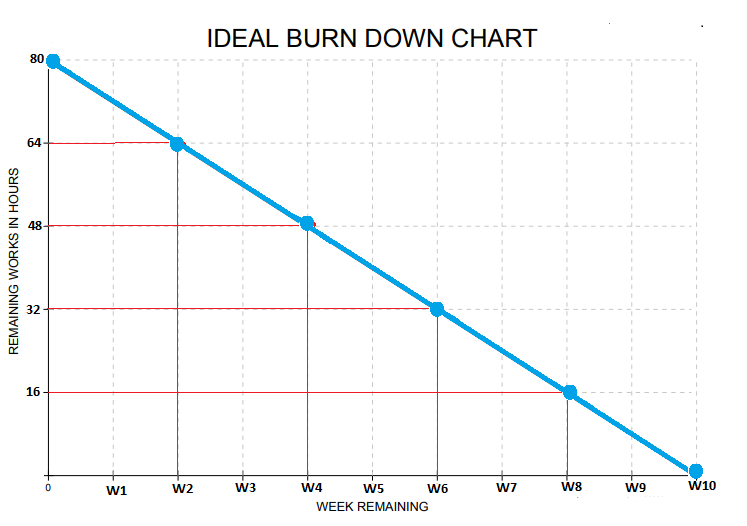
\includegraphics[width=.9\textwidth]{BURDOWNEDITED.PNG}
\caption{Ideal burndown chart}
\end{figure}

\subsubsection{GitHub Registration}
GitHub is an online-browser based distributed version control system for software developers using the Git revision control system. The service provides free public repositories, issue tracking, graphs, code review, downloads, wikis, collaborator management, and more.GitHub offers free accounts for users and organizations working on public and open source projects, as well as paid accounts that offer unlimited private repositories and optional user management and security features.Git hub account creation includes the following steps:
 \begin{itemize}
 
 \item Go to the GitHub sign up page,then  Enter a username, valid email address, and password. Use at least one lowercase letter, one numeral, and seven characters.
 \item Review carefully the GitHub Terms of Service and Privacy Policy before continuing and Choose a plan. Hereby anyone can finish the account creation procedure.
 \item  You can store a variety of projects in GitHub repositories, including open source projects. 
 \item In the upper-right corner of any page, click , and then click New repository.
 \item Type a short, memorable name for your repository followed by Optionally, add a description of your repository,public or private repository.
 \item Select Initialize this repository with a README.finally Click Create repository.
 \item After creation, need to collaborate members by the admin. 
 \item In the left sidebar, click Collaborators and teams.
 \item Under "Collaborators",type the name of the person you'd like to give access to the repository, then click Add collaborator.
 \item Next to the new collaborators name, choose the appropriate permission level: Write, Read, or Admin. 
 \item The user will receive an email inviting them to the repository. Once they accept your invitation, they will have collaborator access to your repository.
 \end{itemize} 
 \begin{figure}[hbtp]
%\includegraphics[width=.8\textwidth]{imfc_accumarray} 

\includegraphics[width=1\textwidth]{collaburate}
\caption{Adding Collaborator
}
\end{figure}

 \newpage
 \section{SYSTEM DESIGN}
 System design is the first step in the development phase for any engineering product or system. The term “Design” is defined as “The process of principles for the purpose of defining a processor a system insufficient detail to permit its realization”. And design is most creative and challenging phase of system development life cycle. It is an approach for the creation of the proposed system is designed, which will help in the system coding. System design is vital for efficient database management. It provides the understanding of procedural details necessary for implementing the system. A number of sub- systems are to be identified which constitute the whole system.
Characteristics of well-defined system is\\ \\(1)Acceptability\\ (2)Decision making ability\\ (3)Economy \\(4)Flexibility \\(5)Reliability\\ (6)Simplicity








%}
% \subsection{Network connectivity or any special requirements
%}
%\subsection{Technology}
\subsection{Technology Or Framework}

\subsubsection{Font end:Python}
Python is a widely used general-purpose, high level programming language. It was initially designed by Guido van Rossum in 1991 and developed by Python Software Foundation. It was mainly developed for emphasis on code readability, and its syntax allows programmers to express concepts in fewer lines of code.

Python is a programming language that lets you work quickly and integrate systems more efficiently.

There are two major Python versions- Python 2 and Python 3. Both are quite different.
It is used for:
\begin{enumerate}

\item
web development (server-side),
\item
software development,
\item
mathematics,
\item
system scripting.
\end{enumerate}
\textbf{What can Python do?}
\begin{description}[font=$\bullet$]
\item
Python can be used on a server to create web  applications.
\item
Python can be used alongside software to create workflows.
\item
Python can connect to database systems. It can also read and modify files.
\item
Python can be used to handle big data and perform complex mathematics.
\item
Python can be used for rapid prototyping, or for production-ready software development.
\end{description}
\textbf{Why Python?}
\begin{description}[font=$\bullet$]
\item
Python works on different platforms (Windows, Mac, Linux, Raspberry Pi, etc).
\item
Python has a simple syntax similar to the English language.
\item
Python has syntax that allows developers to write programs with fewer lines.
\item
Python runs on an interpreter system,so the code can be executed as soon as it is written.
\item
Python can be treated in a procedural way, an object-orientated way or a functional way.
\end{description}
\subsubsection{Back end:MySQL}
MySQL is an open-source relational database management system that works on many platforms. It provides multi-user access to support many storage engines and is backed by Oracle. So, you can buy a commercial license version from Oracle to get premium support services.
\begin{description}[font=$\bullet$]
\item
\textbf{Ease of Management}
\\The software very easily gets downloaded and also uses an event scheduler to schedule the tasks automatically.
\item
\textbf{Robust Transactional Support}
\\
Holds the ACID (Atomicity, Consistency, Isolation, Durability) property, and also allows distributed multi-version support. 
\item
\textbf{Comprehensive Application Development}\\ MySQL has plugin libraries to embed the database into any application. It also supports stored procedures, triggers, functions, views and many more for application development. You can refer to the RDS Tutorial, to understand Amazon’s RDBMS. 
\item
\textbf{
High Performance }\\Provides fast load utilities with distinct memory caches and table index partitioning.
\item
\textbf
{Low Total Cost Of Ownership}\\ This reduces licensing costs and hardware expenditures.
\item
\textbf{Secure Data Protection}\\ MySQL supports powerful mechanisms to ensure that only authorized users have access to the databases.
\item
\textbf{High Availability} MySQL can run high-speed master/slave replication configurations and it offers cluster servers.
\item
\textbf{Scalability and Flexibility } With MySQL you can run deeply embedded applications and create data warehouses holding a humongous amount of data.
\end{description}
\subsubsection{Framework:Django}
Django is a Python-based web framework which allows you to quickly create web application without all of the installation or dependency problems that you normally will find with other frameworks.
\\
When you’re building a website, you always need a similar set of components: a way to handle user authentication (signing up, signing in, signing out), a management panel for your website, forms, a way to upload files, etc. Django gives you ready-made components to use.
\begin{enumerate}
\item
It’s very easy to switch database in Django framework.
\item
It has built-in admin interface which makes easy to work with it.
\item
Django is fully functional framework that requires nothing else.
\item
It has thousands of additional packages available.
\item
It is very scalable.
\end{enumerate}
 Here are few advantages of using Django which can be listed out here :
	\begin{itemize}
	\item \textbf{Object-Relational Mapping (ORM) Support:} Django provides a bridge between the data model and the database engine, and supports a large set of database systems including MySQL, Oracle, Postgres, etc. Django also supports NoSQL database through Django-non rel fork. For now, the only NoSQL databases supported are MongoDB and google app engine. 
	\item \textbf{Multilingual Support:}	 Django supports multilingual websites through its built-in internationalization system. So you can develop your website, which would support multiple languages.
	\item \textbf{Framework Support:} Django has built-in support for Ajax, RSS, Caching and various other frameworks.
	\item \textbf{Administration GUI:} Django provides a nice ready-to-use user interface for administrative activities.
	\item \textbf{Development Environment:} Django comes with a lightweight web server to facilitate end-to-end application development and testing.

\end{itemize}
\subsubsection{GIT- Version ontrol}
\fontsize{12pt}{12pt}\selectfont
\textbf{Version Control System}
\paragraph{} A version control system (VCS) allows you to track the history of a collection of files. It supports creating different versions of this collection. Each version captures a snapshot of the files at a certain point in time and the VCS allows you to switch between these versions. These versions are stored in a specific place, typically called a repository.\newline 
\\
\textbf{Localized and Centralized VCS}
\paragraph*{} A localized version control system keeps local copies of the files. This approach can be as simple as creating a manual copy of the relevant files.
\paragraph*{}
A centralized version control system provides a server software component which stores and manages the different versions of the files. A developer can copy (checkout) a certain version from the central sever onto their individual computer.
\\

\textbf{Distributed VCS}
\paragraph*{} In a distributed version control system each user has a complete local copy of a repository on his individual computer. The user can copy an existing repository. This copying process is typically called cloning and the resulting repository can be referred to as a clone.Every clone contains the full history of the collection of files and a cloned repository has the same functionality as the original repository. \\\\
\textbf{Git}
\paragraph*{}
Git is currently the most popular implementation of a distributed version control system.Git originates from the Linux kernel development and was founded in 2005 by Linus Torvalds. Nowadays it is used by many popular open source projects, e.g., the Android or the Eclipse developer teams, as well as many commercial organizations.The core of Git was originally written in the programming language C, but Git has also been re-implemented in other languages, e.g., Java, Ruby and Python.
\newpage
\subsection{Module Description}
\fontsize{12pt}{12pt}\selectfont
In this Project we have 4 main modules:

\subsubsection{Face Deectin and Recognition}
\begin{itemize}\item
Face detection is defined as finding the position of the face of an individual. In other word it can be defined as locating the face region in an image. \item
After detecting the face of human its facial features is extracted and has wide range of application like facial expression recognition ,face recognition, observation systems, human PC interface and so forth…Detecting face in an image of single person is easy but when we consider a group image of an image containing multiple faces, the task becomes difficult.
\end{itemize}
\subsubsection{Admin Module}
\fontsize{12pt}{12pt}\selectfont
Main fuctions of admin module is listed below: 
 \begin{itemize}
	\item Login
	\item Viewing all registered users details
	\item Add Faculty
\end{itemize}

\subsubsection{Student Module}
\fontsize{12pt}{12pt}\selectfont
Main fuctions of student module is listed below: 
\begin{itemize}
	\item Registration and Login
	\item Get warning of low attendance
	\item Viewing Subject wise atendance
\end{itemize}

\subsubsection{Faculty Module}
\fontsize{12pt}{12pt}\selectfont
Main fuctions of Faculty module is listed below: 
\begin{itemize}
	\item Login
	\item Mark period details so it can record students attendance for respected subject
	\item Viewing time table and attendance status
\end{itemize}

\newpage
\subsection{TABLE DESIGN}

\includegraphics{student.png}

\includegraphics[width=.9\textwidth]{login1.png}
\paragraph{}
\includegraphics[width=.9\textwidth]{f1}
\newpage
\includegraphics{att.png}
\newpage
\subsection{Input Design}
\fontsize{12pt}{12pt}\selectfont
\paragraph{}
Input design converts user-oriented inputs to computer- based format, which requires careful attention. The collection of input data is the most expensive part of the system in terms of the equipment used and the number of people involved. In input design, data is accepted for computer processing and input to the system is done through mapping via some map support or links.The input screens need to be designed very carefully and logically. A set of menus is provided which help for better application navigation. While entering data in the input forms, proper validation checks are done and messages will be generated by the system if incorrect data has been entered.
\paragraph{}
In this project,each module have its own input screens and value insert from option box.For ex
ample,result page will display results of students.
\fontsize{14pt}{14pt}\selectfont
\subsection{Database Design}
\fontsize{12pt}{12pt}\selectfont
\paragraph{}
Data design is the first and most important design activity. Here the main issue is to select the appropriate data structure. That is the Data design focuses on the definition of data structures.
\paragraph{}
Database design is required to manage the large bodies of information. The management of data involves both the definition of structure of the storage information and provisions of mechanism for the manipulation of information. In addition the database system must provide for the safety of information handled, despite the system crashes due to attempts art unauthorized access. For developing an efficient database, we will have to fulfill certain condition such as:\\
\fontsize{12pt}{12pt}\selectfont
\textbf{- }Control redundancy.\\
\textbf{- }Ease of use.\\
\textbf {- }Data independence.\\
\textbf{- }Accuracy and integrity.\\
\textbf{- }Avoiding in ordinate delays.\\
\textbf{- }Recovery from failure.\\
\textbf{- }Privacy and security.\\
\\
\textbf{Normalization}
\paragraph{}
The process of normalization is concerned with the transformation of the conceptual schema to a
computer represent able form. Normalization reduces the redundancies and anomalies
\\
\\
\textbf{First Normal Form}
\paragraph{}
First normal form does not allow multi valued and composite valued attributes. It states that the
domain of an attribute must include only atomic values and that value of any attribute in a tuple must
be single value from the domain of that attribute.
\\
\\
\textbf{Second Normal Form}
\paragraph{}
Second normal form is a normal form used in database normalization. 2NF was originally defined
by E.F. Codd in 1971. To qualify for second normal form a relation must: be in first normal form not
have any non-prime attribute that is dependent on any proper subset of any candidate key of the relation.
\\
\\
\textbf{Third Normal Form}
\paragraph{}
The third normal form (3NF) is a normal form used in database normalization. Third normal form
(3NF) is a normal form that is used in normalizing a database design to reduce the duplication of
data and ensure referential integrity by ensuring that the entity is in second normal form no non-prime
(non-key) attribute is transitively dependent of any key i.e. no non-prime attribute depends on other
non-prime attributes. All the non-prime attributes must depend on the primary key only.
\fontsize{14pt}{14pt}\selectfont
\subsection{Output Design}
\fontsize{12pt}{12pt}\selectfont
\paragraph{}
Outputs are the most important a direct source of information to the user and to the department. Intelligent output design will improve the systems relationship with the user and help much indecision-making. Outputs are so used to provide a permanent hard copy of the results for later uses. The forms used in the system are shown in the appendix. Computer output is the most important and direct source of information the user. Efficient, intelligible output design should improve the systems relationship with the user and help in decision making.

\fontsize{14pt}{14pt}\selectfont
\subsection{User Interface Design}
\fontsize{12pt}{12pt}\selectfont
\paragraph{}
User interface design or user interface engineering is the design of user interfaces for machines and software, such as computers, home appliances, mobile devices, and other electronic devices, with the focus on maximizing usability and the user experience. The goal of user interface design is to make the user's interaction as simple and efficient as possible, in terms of accomplishing user goals.
\paragraph{}
Good user interface design facilitates finishing the task at hand without drawing unnecessary attention to itself. Graphic design and typography are utilized to support its usability, influencing how the user performs certain interactions and improving the aesthetic appeal of the design; design aesthetics may enhance or detract from the ability of users to use the functions of the interface. The design process must balance technical functionality and visual elements to create a system that is not only operational but also usable and adaptable to changing user needs.



\subsection{Hardware and Software Specification
}\subsection{Hardware Specification}
The most common set of requirements defined by any operating system or software application is the physical computer resources, also known as hardware, A hardware requirements list
is often accompanied by a hardware compatibility list (HCL), especially in case of operating
systems. An HCL lists tested, compatible, and sometimes incompatible hardware devices for a
particular operating system or application.\paragraph{}

\includegraphics[width=.8\textwidth]{hardware}


\subsection{Software Specification}

OpenCV (Open Source Computer Vision Library) is an open source computer vision and machine learning software library. OpenCV was built to provide a common infrastructure for
computer vision applications and to accelerate the use of machine perception in the commercial products. Being a BSD-licensed product, OpenCV makes it easy for businesses to utilize
and modify the code. The library has more than 2500 optimized algorithms, which includes a
comprehensive set of both classic and state-of-the-art computer vision and machine learning algorithms. These algorithms can be used to detect and recognize faces, identify objects, classify
human actions in videos, track camera movements, track moving objects, extract 3D models
of objects, produce 3D point clouds from stereo cameras, stitch images together to produce a
high resolution image of an entire scene, find similar images from an image database, remove
red eyes from images taken using flash, follow eye movements, recognize scenery and establish
markers to overlay it with augmented reality, etc. OpenCV has more than 47 thousand people of
user community and estimated number of downloads exceeding 7 million. The library is used
extensively in companies, research groups and by governmental bodies.\paragraph{}
As an asynchronous event driven framework, Node.js is designed to build scalable network
applications. In the following "hello world" example, many connections can be handled concurrently. Upon each connection the callback is fired, but if there is no work to be done Node is
sleeping.\paragraph{}
MySQL is the world’s most popular open source database. With its proven performance, reliability and ease-of-use, MySQL has become the leading database choice for web-based applications, used by high profile web properties.\paragraph{}
Oracle drives MySQL innovation, delivering new capabilities to power next generation web,
cloud, mobile and embedded applications.




%\newpage
%\section{CODING}
\newpage
\section{TESTING}
Testing helps not only to uncover errors introduced during coding, but also locates errors committed during the previous phases. Thus the aim of testing is to uncover requirements, design or coding errors in the program. Software Testing is a critical element of software quality assurance and represents the ultimate review of specification, design and coding,Testing present interesting anomaly for the software engineer.
\subsection{Unit testing}
This is the first of testing. In this different modules are tested against the specification produces during the design of the modules. It refers to the verification of single program module in an isolated environment. Unit testing focuses on the modules independently of one another to locate errors.\paragraph{}
In our project we test each module and each forms individually. Each forms may tested us- ing appropriate values. The input screens need to be designed very carefully and logically.While entering data in the input forms, proper validation checks are done and messages will be gener- ated by the system if incorrect data has been entered.
\subsection{Validation Testing}
The process of evaluating software during the development process or at the end of the development process to determine whether it satisfies specified business requirements. Validation Testing ensures that the product actually meets the client's needs.\paragraph{}
 It can also be defined as to demonstrate that the product fulfills its intended use when deployed on appropriate environment.
\subsection{System Testing}
System Testing is the testing of a complete and fully integrated software product. Usually, software is only one element of a larger computer-based system. Ultimately, software is interfaced with other software/hardware systems. System Testing is actually a series of different tests whose sole purpose is to exercise the full computer-based system.
\newpage
\section{IMPLEMENTATION}
The system uses Viola Jones algorithm for face detection and PCA algorithm for face
recognition.
\subsection{Viola Jones Algorithm}
The Viola–Jones object detection framework is the first object detection framework to
provide competitive object detection rates in rea ltime proposed in 2001 by Paul Viola and
Michael Jones. Although it can be trained to detect a variety of object classes, it was motivated
primarily by the problem of face detection. The characteristics of Viola–Jones algorithm which
make it a good detection algorithm are:
\begin{enumerate}

\item
 Robust – very high detection rate (true positive rate) and very low false positive rate
always.
\item
Real time – For practical applications at least 2 frames per second must be processed.
\end{enumerate}
\paragraph{}
Face detection only (not recognition) The goal is to distinguish faces from nonfaces (detection is the first step in the recognition process).There are three major blocks in Viola Jones
algorithm, Integral Images, AdaBoost Algorithm and Attentional cascade. The integral image
computes a value at each pixel for example (x, y) that is the sum of the pixel values above to the
left of ()x, y). This is quickly computed in one pass through the image. Viola jones algorithm
uses Haar like features. This is nothing but scalar product between the image and some haar
like structures. Feature is selected through adaboost. AdaBoost provides an effective learning
algorithm and strong bounds on generalization performance. The overall form of the detection
process is that of a degenerate decision tree, what we call a “cascade”. A positive result from
the first classifier triggers the evaluation of a second classifier which has also been adjusted to
achieve very high detection rates. A positive result from the second classifier triggers a third
classifier, and so on. A negative outcome at any point leads to the immediate rejection of the sub
window. The cascade training process involves two types of tradeoffs. In most cases classifiers
with more features will achieve higher detection rates and lower false positive rates. At the
same time classifiers with more features require more time to compute. In principle one can use
following stages.
\\i) the number of classifier stages, ii) the number of features in each stage, and iii) the
threshold of each stage, are traded off in order to minimize the expected number of evaluated
features.\paragraph{}
The basic principle of the Viola-Jones algorithm is to scan a sub-window capable of detecting faces across a given input image. The standard image processing approach would be
to rescale the input image to different sizes and then run the fixed size detector through these
images. This approach turns out to be rather time consuming due to the calculation of the
different size images.\paragraph{}
Contrary to the standard approach Viola-Jones rescale the detector instead of the input
image and run the detector many times through the image – each time with a different size.
At first one might suspect both approaches to be equally time consuming, but Viola-Jones have
devised a scale invariant detector that requires the same number of calculations whatever the
size. This detector is constructed using a so-called integral image and some simple rectangular
features reminiscent of Haar wavelets. The next section elaborates on this detector.\\
\textbf{The scale invariant detector:} The first step of the Viola-Jones face detection algorithm
is to turn the input image into an integral image. This is done by making each pixel equal to
the entire sum of all pixels above and to the left of the concerned pixel. This is demonstrated
in figure 2.\\
\includegraphics{a1}\paragraph{}
This allows for the calculation of the sum of all pixels inside any given rectangle using only
four values. These values are the pixels in the integral image that coincide with the corners of
the rectangle in the input image. This is demonstrated in Figure 3.


\includegraphics{a2}
\paragraph{}
Since both rectangle B and C include rectangle A the sum of A has to be added to the
calculation. It has now been demonstrated how the sum of pixels within rectangles of arbitrary
size can be calculated in constant time. The Viola-Jones face detector analyzes a given subwindow using features consisting of two or more rectangles. The different types of features are
shown in Figure 4.
\\
\includegraphics{a3}
\paragraph{}
Each feature results in a single value which is calculated by subtracting the sum of the
white rectangle(s) from the sum of the black rectangle(s).\paragraph{}
Viola-Jones have empirically found that a detector with a base resolution of 24*24 pixels
gives satisfactory results. When allowing for all possible sizes and positions of the features in
Figure 4 a total of approximately 160.000 different features can then be constructed. Thus, the
amount of possible features vastly outnumbers the 576 pixels contained in the detector at base
resolution. These features may seem overly simple to perform such an advanced task as face
detection, but what the features lack in complexity they most certainly have in computational
efficiency.\paragraph{}
One could understand the features as the computer’s way of perceiving an input image.
The hope being that some features will yield large values when on top of a face. Of course
operations could also be carried out directly on the raw pixels, but the variation due to different
pose and individual characteristics would be expected to hamper this approach.\\
\textbf{title The modified AdaBoost algorithm:} As stated above there can be calculated
approximately 160.000 feature values within a detector at base resolution. Among all these features some few are expected to give almost consistently high values when on top of a face.
In order to find these features Viola-Jones use a modified version of the AdaBoost algorithm
developed by Freund and Schapire in 1996.
AdaBoost is a machine learning boosting algorithm capable of constructing a strong classifier through a weighted combination of weak classifiers. (A weak classifier classifies correctly
in only a little bit more than half the cases.) To match this terminology to the presented theory
each feature is considered to be a potential weak classifier.
\subsection{PCA Algorithm}
\paragraph{}
The basis of the eigenfaces calculation in this work is the Principal Component Analysis
(PCA).  An objective of PCA is the replacement of correlated vectors of
large dimensions with the uncorrelated vectors of smaller dimensions. Another objective is to
calculate a basis for the data set. Main advantages of the PCA are its low sensitivity to noise, the
reduction of the requirements of the memory and the capacity, and the increase in the efficiency
due to the operation in a space of smaller dimensions. The strategy of the Eigenfaces method
consists of extracting the characteristic features on the face and representing the face in question
as a linear combination of the so called ‘eigenfaces’ obtained from the feature extraction process.
The principal components of the faces in the training set are calculated. Recognition is achieved
using the projection of the face into the space formed by the eigenfaces. A comparison on the
basis of the Euclidian distance of the eigenvectors of the eigenfaces and the eigenface of the
image under question is made. If this distance is small enough, the person is identified.  As a starting point, the training images of
dimensions N*N are read and they are converted to N2 *1 dimensions. A training set of N2 *M
dimensions is thus created, where M is the number of sample images.
The eigenfaces corresponding to the highest eigenvalues are retained. Those eigenfaces
define the face space. The eigenspace is created by projecting the image to the face space
formed by the eigenfaces. Thus the weight vectors are calculated. Dimensions of the image
are adjusted to meet the specifications and the image is enhanced in the preprocessing steps of
recognition. The weight vector of the image and the weight vectors of the faces in the database
are compared. Average face is calculated and subtracted from each face in the training set. A
matrix (A) is formed using the results of the subtraction operation. The dimensions of the matrix
C is N*N. M images are used to form C. In practice, the dimensions of C is N*M. On the other
hand, since the rank of A is M, only M out of N eigenvectors are nonzero. 
\paragraph{}
The eigenvalues of the covariance matrix is calculated. The eigenfaces are created by using the number of training
images minus number of classes (total number of people) of eigenvectors. The selected set of
eigenvectors are multiplied by the A matrix to create a reduced eigenface subspace.\\
Steps used in PCA face recognition:-
\begin{enumerate}

\item
Acquire training set of ‘N’ number of images at the initial stage.
\item
Calculation of the eigen face from the “N” training set images keeping only few M images
that is correspond to that of the highest eigen values. The M images describe the “face
space”. When new faces encountered, the “eigen faces” can be recalculated accordingly.
\item
The corresponding distribution of the “M” dimensional weight space for every known
individual is Calculated by projecting their respective face images onto “face space”.
\item
Compute set of the weights anticipating or projecting the data picture or input image to
M “eigen faces”.
\item
Determine if the given image is face image or not by checking to the closeness of given
image or picture to “face space”.
\item
If the image is sufficiently close enough, then classify the weight pattern as either an
unknown or as a known person based on measured Euclidean distance.
\item
If the image is sufficiently close enough then refer to the recognition is successful and give
applicable information about recognized face from the database which hold data of faces.
\end{enumerate}
%\newpage
%\section{FUTURE SCOPE OR ENHANCEMENT}
\newpage
\section{FUTURE SCOPE}
It can be easily implemented at any institute or organization. A method could be proposed toillustrate robustness against the variations that is, in near future we could build a system which would be robust and would work in undesirable conditions too. Here it is proposed for an institute to take the attendance of the students but in future it can be used to do the same work at entry as well as exit points. Authors are working to improve the face recognition effectiveness to build more efficient sys- tems in near future.\paragraph{} In further work, authors intend to improve face recognition effectiveness by using the interac- tion among our system, the users and the administrators. On the other hand, our system can be used in a completely new dimension of face recognition application, mobile based face recog- nition, which can be an aid for common people to know about any person being photographed by cell phone camera including proper authorization for accessing a centralized database.

\newpage
\section{CONCLUSION}
The automated student attendance system using human face recognition technique works
nicely. The automatic attendance management will replace the traditional method, which takes
a lot of time and is hard to maintain. Certainly, it is improved for better result particularly by
paying attention in feature extraction or recognition process.\paragraph{}

This improvement may help the recognition process become more robust. In this system
we have implemented an attendance system by which lecturers or teaching assistants can record
student’s attendance. It saves time and effort, especially if it is a lecture with huge number of
students. Another application of this system is that it is capable of marking the presence of
employees at any workplace. The system can be useful in many other areas and can replace the
existing systems of attendance marking.\paragraph{}

Face recognition technologies have been associated generally with very costly top secure
applications. Today the care technologies have evolved and the cost of equipment is going down
dramatically due to the integration.




%======================================================================







%\fontsize{12pt}{12pt}\selectfont
  % \lstinputlisting{git1.txt}
%\fontsize{15pt}{15pt}\selectfont

%\subsection{Screen Shots Of Forms,Reports,Diagrams(Burn down charts}
%\subsection{Sample templates for Sprint Backlog, Daily scrum etc.
%}
%\subsection{Sample code}



%==========================================================================
\newpage
\section{APPENDIX}
\subsection{Git History }	
		\fontsize{12pt}{12pt}\selectfont
				
				\begin{lstlisting}
JOISKJ@HP MINGW64 ~
$ mkdir miniproject		
JOISKJ@HP MINGW64 ~
$ cd miniproject
JOISKJ@HP MINGW64 ~/miniproject
$ mkdir attendance
JOISKJ@HP MINGW64 ~/miniproject
$ cd attendance
		
JOISKJ@HP MINGW64 ~/miniproject/attendance
$ mkdir attendance
		
JOISKJ@HP MINGW64 ~/miniproject/attendance
$ cd attendance
JOISKJ@HP MINGW64 ~/miniproject/attendance/attendance
$ git init
Initialized empty Git repository in C:/Users/JOISKJ/miniproject/attendance/attendance/.git/
JOISKJ@HP MINGW64 ~/miniproject/attendance/attendance (master)
$ git config --global user.name "varna"
JOISKJ@HP MINGW64 ~/miniproject/attendance/attendance (master)
$ git config --global user.email "varnablal2108@gmail.com"
JOISKJ@HP MINGW64 ~/miniproject/attendance/attendance (master)
$ git clone https://github.com/varnablal/attendance
Cloning into 'attendance'...
remote: Enumerating objects: 135, done.
remote: Total 135 (delta 0), reused 0 (delta 0), pack-reused 135
Receiving objects: 100% (135/135), 4.13 MiB | 769.00 KiB/s, done.
Resolving deltas: 100% (28/28), done.
JOISKJ@HP MINGW64 ~/miniproject/attendance/attendance (master)
$ git add .
JOISKJ@HP MINGW64 ~/miniproject/attendance/attendance (master)
$ git commit -m "Sprint 1 Commited"
[master (root-commit) 8a971c6] Sprint 1 Commited
1 file changed, 1 insertion(+)
create mode 160000 Illicit-Drug
		
$ git push origin master
Username for 'https://github.com':varnablal
Password for 'https://varnablal2108@github.com': 
Counting objects: 5, done.
Delta compression using up to 2 threads.
Compressing objects: 100 (3/3), done.
Writing objects: 100 (4/4), 944 bytes | 0 bytes/s, done.
Total 4 (delta 0), reused 0 (delta 0)
To https://github.com/E/minproject/attendance/attendance 
94cf147..c55d152  master -> master
JOISKJ@HP MINGW64 ~/miniproject/attendance/attendance (master)
		

		\end{lstlisting}	
%\includegraphics[width=1\textwidth]{git11}
%\newpage
%\includegraphics[width=.9\textwidth]{gita1b}
%\paragraph{}
%\hspace{.5cm}\includegraphics[width=1.1\textwidth]{a1b}
\newpage
\subsection{Sample Code}
\begin{lstlisting}

# import the libraries
	import os
	import face_recognition
	import cv2
	# make a list of all the available images
	#images = os.listdir(os.path.join(os.getcwd(),'Facelive\images'))
	ta=os.getcwd()
	images = os.listdir(os.path.join(ta,'camera/images'))
	images111 = os.path.join(ta,'camera/images')
	print(images111)
	font = cv2.FONT_HERSHEY_DUPLEX
	bottomLeftCornerOfText = (10, 400)
	fontScale = .5
	fontColor = (0, 0, 255)
	lineType = 1

	myPath = 'Facelive'
	print('Creating the haar cascade...')
	cascPath = os.path.join(myPath, 'haarcascades',
\end{lstlisting}
\begin{lstlisting}	
	 'haarcascade_frontalface_default.xml')
	faceCascade = cv2.CascadeClassifier(cascPath)
	attendance=[]
	def most_frequent(List): 
		counter = 0
		num = List[0] 
		
		for i in List: 
			curr_frequency = List.count(i) 
			if(curr_frequency> counter): 
				counter = curr_frequency 
				num = i 
	
		return num 
	
	List = [2, 1, 2, 2, 1, 3] 
	print(most_frequent(List)) 
	def current_minute():
		import time
		t = time.localtime()
		current_time = time.strftime("%H:%M:%S", t)
		data = current_time.split(':')
		return data[1]

	res1 = current_minute()
	print('Setting up camera...')
	cam = cv2.VideoCapture(0)
	lii=[]
	while True:
		res = current_minute()
		ret,frame = cam.read()

		k = cv2.waitKey(1)
		if k % 256 == 27:
			# ESC pressed
			print("Escape hit, closing...")
			break
		# load the example image and convert it to grayscale
		image = frame
		gray = cv2.cvtColor(image, cv2.COLOR_BGR2GRAY)
		
		# Detect faces in the image
		faces = faceCascade.detectMultiScale(
			gray,
			scaleFactor=1.1,
			minNeighbors=5,
			minSize=(30, 30),
			flags=cv2.CASCADE_SCALE_IMAGE)
		#     There is only 1 driver. So consider only 1 detection

		if len(faces) == 0:
			continue
		
		face = [faces[0]]    
		# Draw a rectangle around the faces
		for (x1, y1, w, h) in face:
			cv2.rectangle(frame, (x1, y1), (x1 + w, y1 + h), 
			(0, 255, 0), 2)
			sub_face = frame[y1:y1+h, x1:x1+w]
		cv2.imshow('Webcam',frame)        


		filename = "{}.jpg".format(os.getpid())
		cv2.imwrite(filename, sub_face)


		image_to_be_matched = 
		face_recognition.load_image_file(filename)

		try:
			# encoded the loaded image into a feature vector
			img_encoded= face_recognition.face_encodings
			(image_to_be_matched)[0]
		except IndexError:
			continue
		
		# iterate over each image
		for image in images:
			# load the image
			current_image = face_recognition.load_image_file
			(images111 +'/'+ image)
			# encode the loaded image into a feature vector
			current_image_encoded=
			face_recognition.face_encodings
			(current_image)[0]
			
			result = face_recognition.compare_faces(
				[img_encoded], current_image_encoded)
			
			# check if it was a match
			if result[0] == True:
				im = image[:-4]
				im = im.upper()
				
				lii.append(im)
			# print(lii)
			if len(lii)>10:
			  attendance.append(most_frequent(lii))
			  lii=[]
			print(res)        
				
			if int(res)==int(res1)+1:
				
				cam.release()
				cv2.destroyAllWindows()
				return attendance
				attendance=[]
				cam.release()
				cv2.destroyAllWindows()
				exit()
				
					

					
				
			#else:
				#print("Not matched: ",image)
	# When everything done, release the capture
	#cap.release()
	cv2.destroyAllWindows()
	#Returns the captured image's name
	print('Saved.')





\end{lstlisting}












\subsection{Screen Shots of Forms
}
 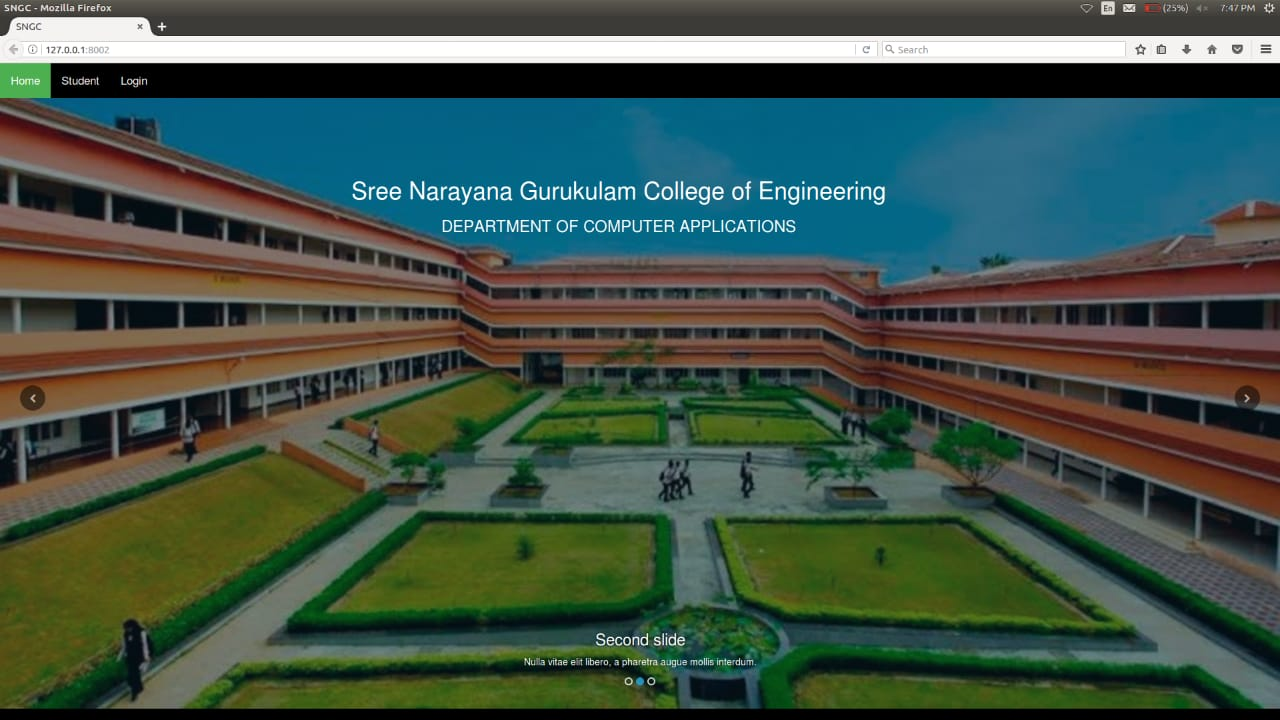
\includegraphics[width=.9\textwidth]{a55}\paragraph{}

     \hspace{5cm}Figure 9.1 Home Page
     \paragraph{}
     \paragraph{}
     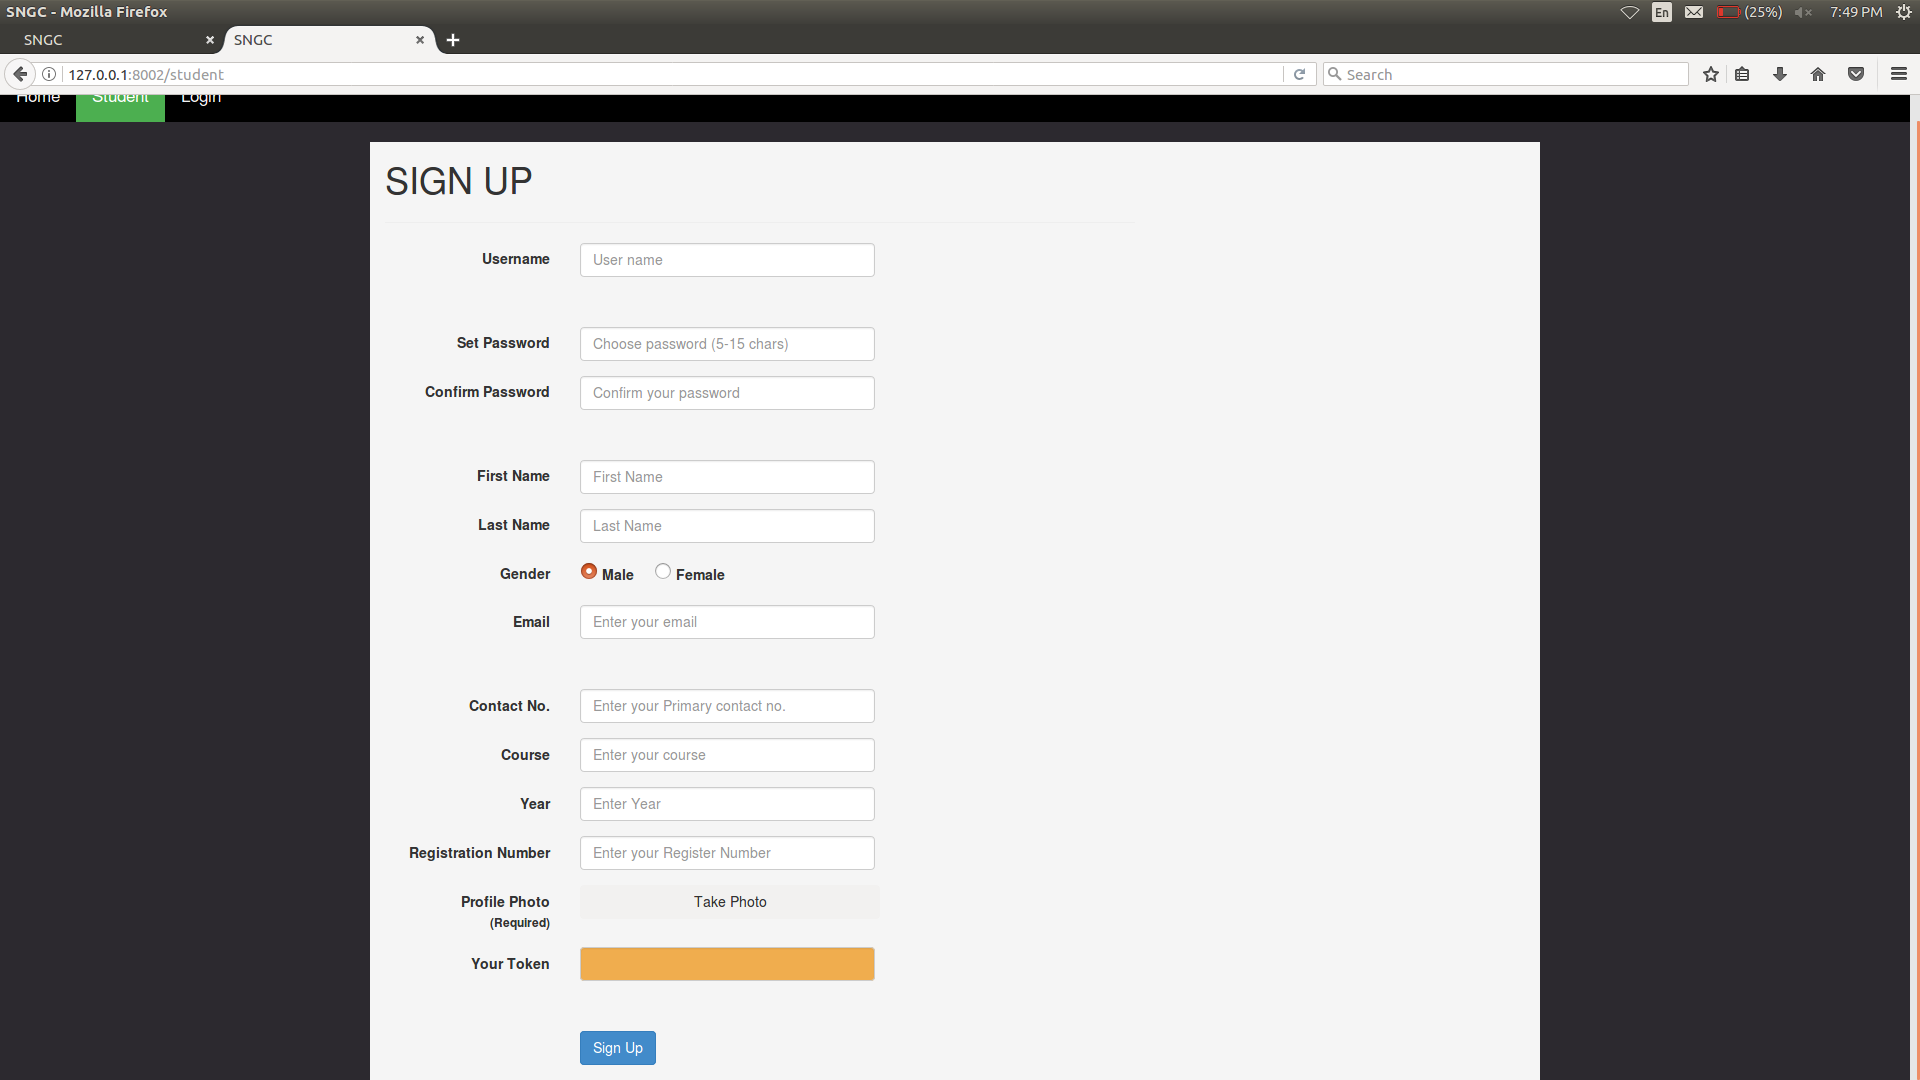
\includegraphics[width=.9\textwidth]{studreg}\paragraph{}
    \hspace{5cm}Figure 9.2 Student Registration
    \newpage
\paragraph{}

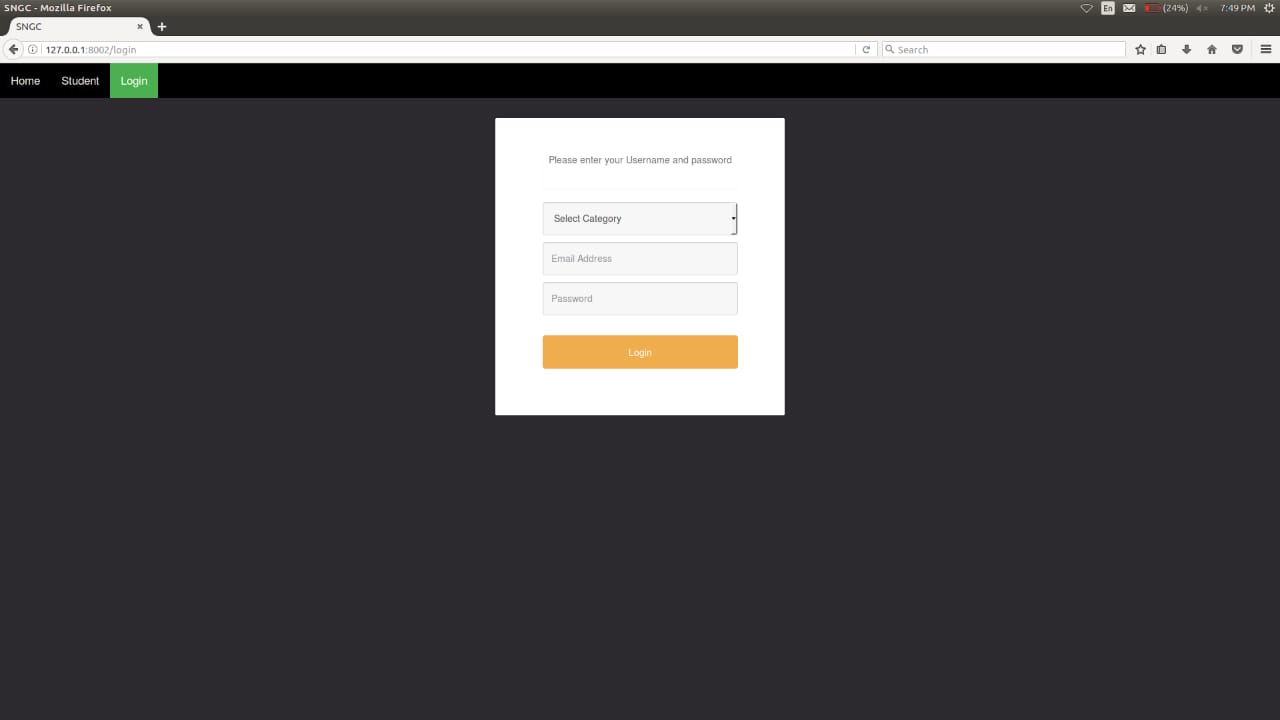
\includegraphics[width=.9\textwidth]{login12}

     \hspace{5cm}Figure 9.3 Login
     \paragraph{}
     
     \includegraphics[width=.9\textwidth]{a77}\paragraph{}
    \hspace{5cm} Figure 9.4 Take Attendance
    
    \newpage
    \paragraph{}
    \includegraphics[width=.9\textwidth]{a66}

     \hspace{5cm}Figure 9.5 Attendance Status
     \paragraph{}
     \paragraph{}
     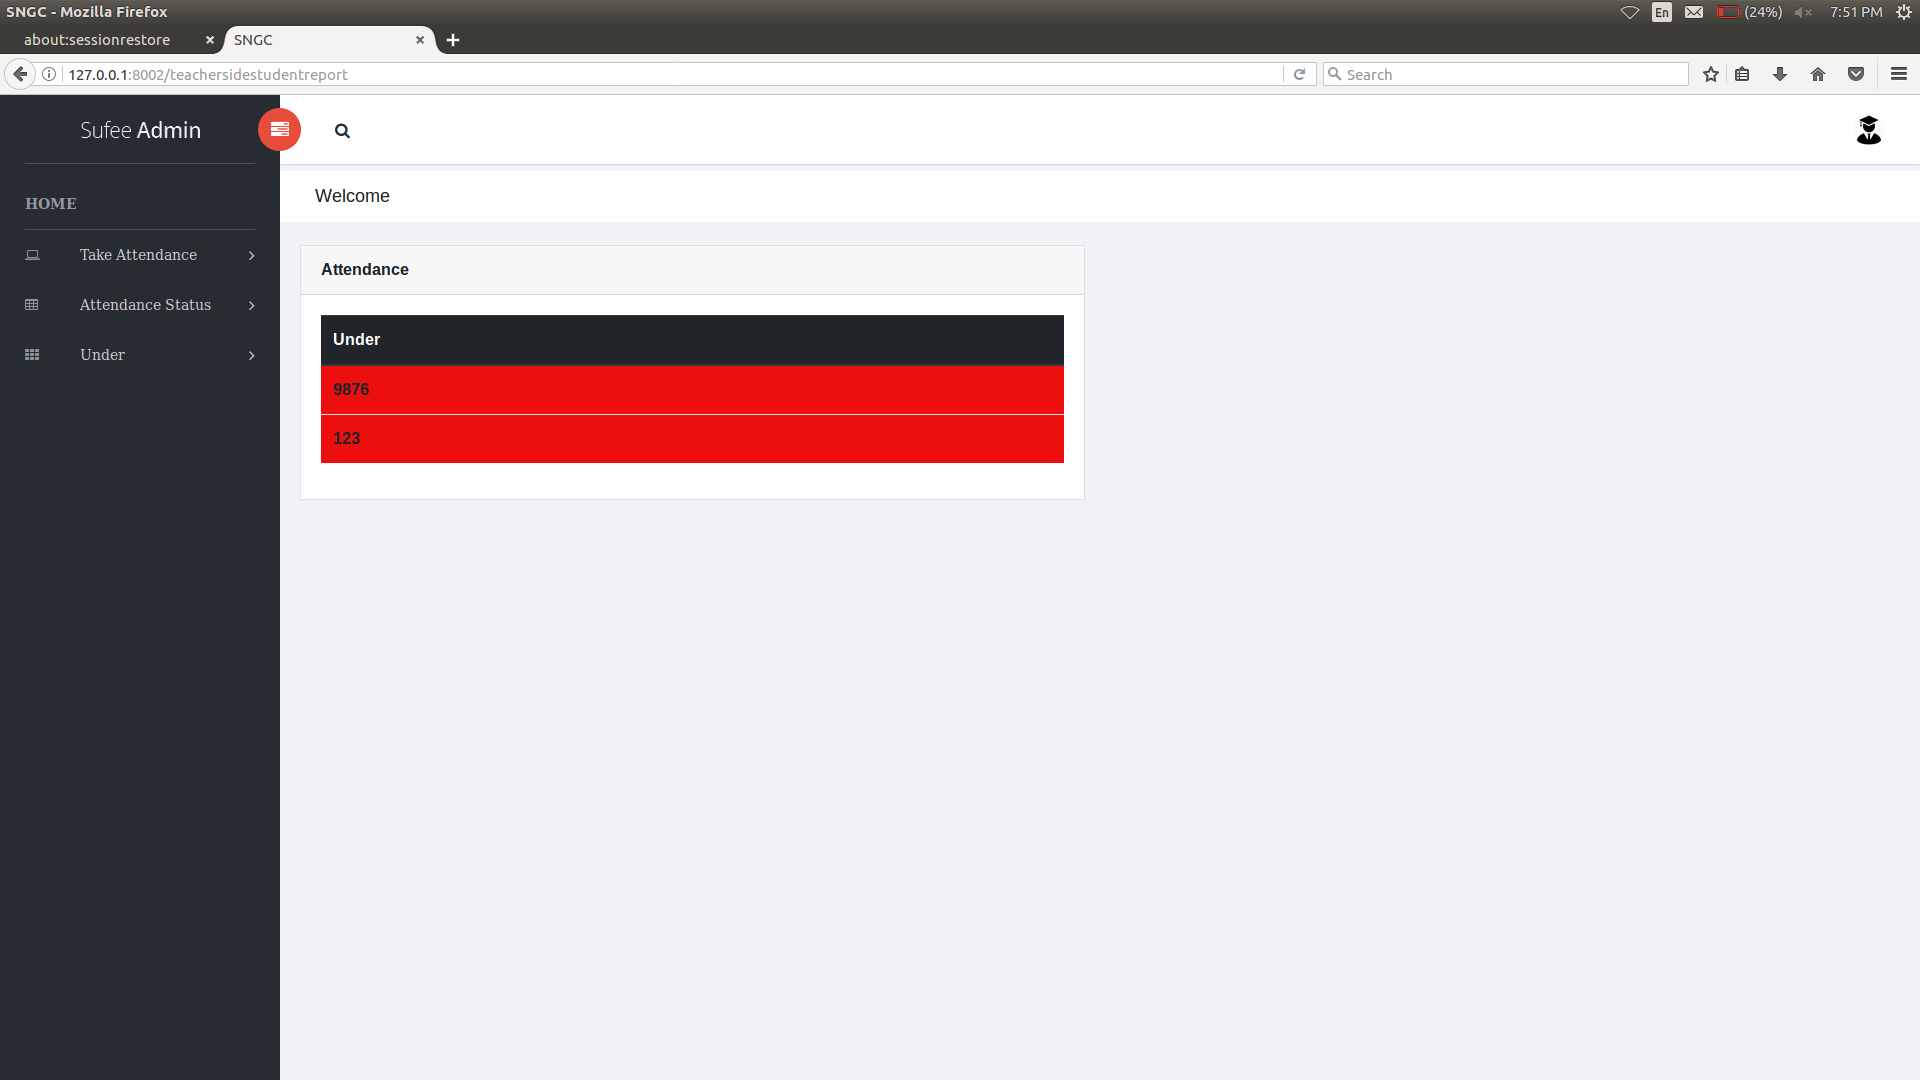
\includegraphics[width=.9\textwidth]{a22}\paragraph{}
    \hspace{5cm}Figure 9.6 Warning Of Low Attendance
    \newpage
    \subsection{Sample Templates For Sprint Backlog,Daily Scrum etc.}
    \paragraph{}
   
    \includegraphics[width=1\textwidth]{t1}
  
     
     \paragraph{}
    \includegraphics[width=1\textwidth]{t2} 
     
   \paragraph{}
     
    \includegraphics[width=1\textwidth]{t3}
    
    \begin{center} 
    Figure 10.1 Sample Template Of Sprint Backlog Of Sprint1
    \paragraph{}
    \end{center}
   
    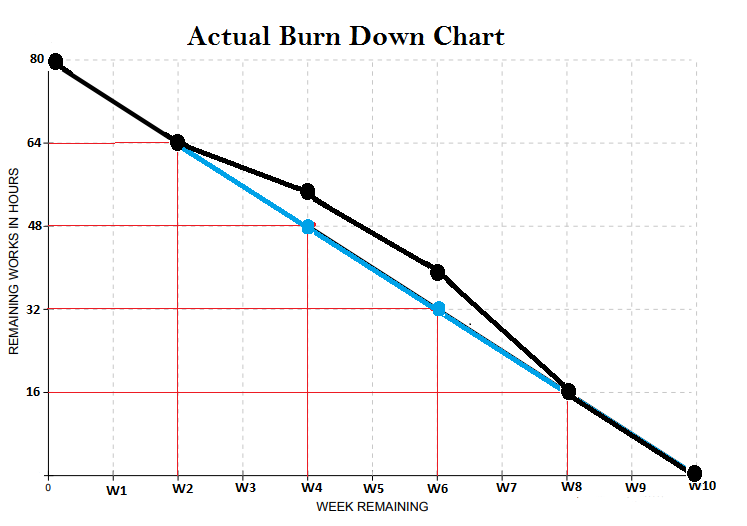
\includegraphics[width=.8\textwidth]{BURDOWNEDITED12}
     \begin{center} 
    Figure 10.2 Actual Burn Down Chart
   
    \end{center}
\newpage
\section{BIBLIOGRAPHY}
\begin{enumerate}[label={$\left[1\right]$}]



\item
 M. A. Turk and A. P. Pentland, “ Face Recognition Using Eigenfaces,”in Proc. IEEE
Conference on Computer Vision and Pattern Recognition, pp. 586–591. 1991.
\end{enumerate}
\begin{enumerate}[label={$\left[2\right]$}]

\item
M. H. Yang, N. Ahuja, and D. Kriegmao, “Face recognition using kernel eigenfaces,”
IEEE International Conference on Image Processing, vol. 1, pp. 1013, Sept. 2000.
\end{enumerate}
\begin{enumerate}[label={$\left[3\right]$}]
\item
Lijuan Duan, Guoqin Cui, Wen Gao and Hongming Zhang“ Adult Image Detection
Method Based on Skin Color Model and Support Vector Machine” ACCV2002: The 5th Asian
Conference on Computer Vision, 2325 January 2002,Melbourne, Australia” .
\end{enumerate}
\begin{enumerate}[label={$\left[4\right]$}]
\item
Arulogun O. T., Olatunbosun, A., Fakolujo O. A., and Olaniyi, O. M. RFID Based
Students Attendance Management System. International Journal of Scientific and Engineering
Research Volume 4, Issue 2, February2013.
\end{enumerate}



\end{document} 